\documentclass[9pt,a4paper,unknownkeysallowed,xcolor=dvipsnames,aspectratio=43]{beamer}
\usepackage{lastpage}
\usepackage{graphicx}
\usepackage{hyperref}  
\usepackage{bm,amsmath,amssymb}

%\usepackage[dvipsnames]{xcolor}
\definecolor{darkred}{RGB}{212, 0, 0}
\definecolor{darkgreen}{RGB}{0,128,0}
\definecolor{teablue}{RGB}{67,0,181}
\definecolor{darkblue}{RGB}{0,0,128}
\hypersetup{
    colorlinks=true,
    linkcolor=blue,
    filecolor=magenta,      
    urlcolor=blue,
    citecolor=blue
}
\newcommand{\currentpage}{\thepage / \pageref{LastPage}}
\setbeamertemplate{footline}
{
  \leavevmode%
  \hbox{%
\footnotesize\sffamily
  \begin{beamercolorbox}[wd=.40\paperwidth,ht=3ex,dp=1ex,center]{}%
   \color{teablue} Jet Physics
  \end{beamercolorbox}%
  \begin{beamercolorbox}[wd=.20\paperwidth,ht=3ex,dp=1ex,center]{}%
  \currentpage 
  \end{beamercolorbox}%
  \begin{beamercolorbox}[wd=.40\paperwidth,ht=3ex,dp=1ex,center]{}%
   \color{teablue} 6 \& 7. Jet Substructure
  \end{beamercolorbox}%
}
}
\setbeamertemplate{frametitle}[default][center]
\begin{document}


\begin{frame}
\topskip0pt
\vspace*{\fill}
\begin{center}
{\Huge\bf\color{darkred} Introduction to Jet Physics}\\
\vspace{4mm}
    Bin Wu\\
    \vspace{8mm}
    {\bf\Large Lectures 6 \& 7: Jet Substructure}\\\vspace{4mm}
    {\color{darkblue} 21\&22-04-2021}
\end{center}
\vspace{4mm}
\begin{itemize}
    \item[\color{darkred}\Large\bullet] Introduction to jet substructure
    \vspace{2mm}
    \item[\color{darkred}\Large\bullet] Prong-Finders and Groomers
    \vspace{2mm}
    \begin{itemize}
        \item[\diamondsuit] Mass Drop Tagger and Soft Drop
        \vspace{2mm}
        \item[\diamondsuit] Filtering, Trimming and pruning 
        \vspace{2mm}
        \item[\diamondsuit] CMS Top Tagger
    \end{itemize}
    \vspace{2mm}
    \item[\color{darkred}\Large\bullet] Jet Shapes
    \vspace{2mm}
    \begin{itemize}
        \item[\diamondsuit] N-subjettiness
    \end{itemize}
    \vspace{2mm}
    \item[\color{darkred}\Large\bullet] The Lund Jet Plane
    
\end{itemize}
\vspace*{\fill}
\end{frame}
%
%%%%%%%%%%%%%%%%%%%%%%%%%%%%%%%%%%%%%%%%%%%%%%%%%%%%%%%%%%
%
\begin{frame}{\bf\huge Introduction to jet substructure}

{\color{red}The LHC is special:}\\
\vspace{2mm}
%{\color{darkred}\Large$\bullet$}
1. It produces an abundance of highly boosted $W/Z/H$ and top quarks:
\vspace{2mm}
\begin{center}
\includegraphics[width=0.5\textwidth]{05/cms_Z.pdf}\\\vspace{2mm}{

\tiny \color{darkblue}
{\scshape CMS} collaboration,
%\emph{{Measurement of the transverse momentum spectra of weak vector bosons produced in proton-proton collisions at $ \sqrt{s}=8 $ TeV}},
  \href{https://doi.org/10.1007/JHEP02(2017)096}{\emph{JHEP} {\bfseries 02}
  (2017) 096} [\href{https://arxiv.org/abs/1606.05864}{{\ttfamily
  1606.05864}}].
}\\\vspace{2mm}

e.g., about 0.16\% of Z bosons have $p_T = (250-600)$ TeV in this channel!
\end{center}
\end{frame}
%
%
%%%%%%%%%%%%%%%%%%%%%%%%%%%%%%%%%%%%%%%%%%%%%%%%%%%%%%%%%%
%
\begin{frame}

\vspace{2mm}
{\color{darkred}\Large$\bullet$} One can study the $n$-pronged kinematics.

\vspace{2mm}
{\color{darkred}\Large$\bullet$} W Bosons in a single jet
\vspace{1mm}
\begin{center}
\includegraphics[width=0.2\textwidth]{05/Wjet.png}\\\
\vspace{1mm}
\includegraphics[width=0.7\textwidth]{05/semiLepMass_mWCand.pdf}\\%\vspace{2mm}
{\tiny \color{darkblue}{\scshape CMS} collaboration, %\emph{{Search for Anomalous $t\bar{t}$ Production in the Highly-Boosted All-Hadronic Final State}},
  \href{https://doi.org/10.1007/JHEP09(2012)029}{\emph{JHEP} {\bfseries 09}
  (2012) 029} [\href{https://arxiv.org/abs/1204.2488}{{\ttfamily 1204.2488}}].}
\end{center}
\end{frame}
%
%
%%%%%%%%%%%%%%%%%%%%%%%%%%%%%%%%%%%%%%%%%%%%%%%%%%%%%%%%%%
%
\begin{frame}

\vspace{2mm}
{\color{darkred}\Large$\bullet$} Top quarks in a single jet
\vspace{2mm}
\begin{center}
\includegraphics[width=0.2\textwidth]{01/tjets.png}\\\
\vspace{2mm}
\includegraphics[width=0.45\textwidth]{05/tJet.png}\\%\vspace{2mm}
{\tiny \color{darkblue}{\scshape ATlAS} collaboration, %\emph{{Search for Anomalous $t\bar{t}$ Production in the Highly-Boosted All-Hadronic Final State}},
\href{https://cds.cern.ch/record/1571040}{ATLAS-CONF-2013-084};\\
S.~Sch\"atzel, %\emph{{Boosted Top Quarks and Jet Structure}},
  \href{https://doi.org/10.1140/epjc/s10052-015-3636-x}{\emph{Eur. Phys. J. C}
  {\bfseries 75} (2015) 415} [\href{https://arxiv.org/abs/1403.5176}{{\ttfamily
  1403.5176}}].}
\end{center}
\end{frame}
%
%
%%%%%%%%%%%%%%%%%%%%%%%%%%%%%%%%%%%%%%%%%%%%%%%%%%%%%%%%%%
%
\begin{frame}

\vspace{2mm}
%{\color{darkred}\Large$\bullet$}
2. It has large pileup:
\vspace{2mm}
\begin{center}
\includegraphics[width=0.8\textwidth]{05/78pileup.png}\\\vspace{2mm}
{\tiny \color{darkblue}\href{https://cds.cern.ch/record/1479324}{78 reconstructed vertices by CMS}
}\vspace{2mm}

Typically LHC: 20-60\qquad HL-LHC: $\approx$140
\end{center}
\end{frame}
%
%
%%%%%%%%%%%%%%%%%%%%%%%%%%%%%%%%%%%%%%%%%%%%%%%%%%%%%%%%%%
%
\begin{frame}

\vspace{2mm}
{\color{darkred}\Large$\bullet$} Additional soft contamination:
\vspace{2mm}
\begin{center}
\includegraphics[width=0.8\textwidth]{05/tth.pdf}\\\vspace{2mm}
{\color{darkred}Cleaning/grooming is needed!}
\end{center}
\end{frame}
%
%
%%%%%%%%%%%%%%%%%%%%%%%%%%%%%%%%%%%%%%%%%%%%%%%%%%%%%%%%%%
%
\begin{frame}

\vspace{2mm}
{\color{darkred}\Large$\bullet$} {\color{darkred}Categories of jet substructure techniques:}
\vspace{8mm}
\begin{enumerate}
    \item {\color{darkred}Prong finders}: They are invented to look for the number of hard cores in a jet in order to distinguish jets of different origin.
    \vspace{8mm}
    \item {\color{darkred}Groomers:} Large-radius jets are used.Grooming tools aim to remove soft radiation far from the jet axis in order to mitigate the impact of UE and pileup.
    \vspace{8mm}
    \item {\color{darkred}Jet shapes} (radiation constraints): Many jet shapes have been introduced to quantify soft-gluon pattern inside a jet.
\end{enumerate}
\end{frame}
%
%%%%%%%%%%%%%%%%%%%%%%%%%%%%%%%%%%%%%%%%%%%%%%%%%%%%%%%%%%
%
\begin{frame}{\bf\huge Recap: mass distributions for an unstable particle}\vspace{2mm}

{\color{darkred}\Large$\bullet$}: For a {\color{darkred}stable} scalar with mass $m_X$
\begin{align}
&\begin{array}{c}
\includegraphics[width=0.6\textwidth]{05/propagator.png}
\end{array}\notag\\
&=\frac{i}{p^2-m_0^2 + M(p^2)}\approx \frac{i Z}{p^2-m_X^2}\qquad\text{at $p^2\approx m_X^2$}
\end{align}
with
\begin{align}
   m_X^2-m_0^2 + M(m_X^2) =0, \qquad Z = \frac{1}{1 + \left.\frac{d}{dp^2}M(p^2)\right|_{p^2\to m_X^2}}
\end{align}

{\color{darkred}\Large$\bullet$} For an {\color{darkred}unstable} scalar, $M$ obtains an imaginary part. Let us define
\begin{align}
   m_X^2-m_0^2 + \text{Re}~M(m_X^2) =0, \qquad Z = \frac{1}{1 + \left.\frac{d}{dp^2}\text{Re}~M(p^2)\right|_{p^2\to m_X^2}}.
\end{align}
Accordingly, at $p^2\approx m_X^2$
\begin{align}
\begin{array}{c}
\includegraphics[width=0.15\textwidth]{05/propagatorun.png}
\end{array}
\approx \frac{i Z}{p^2-m_X^2 + i Z \text{Im}~M(p^2)}
\end{align}
\end{frame}
%
%%%%%%%%%%%%%%%%%%%%%%%%%%%%%%%%%%%%%%%%%%%%%%%%%%%%%%%%%%
%
\begin{frame}\vspace{2mm}

{\color{darkred}\Large$\bullet$} The optical theorem:
\begin{align}
1 = S^\dagger S \Rightarrow -i (T - T^\dagger)\qquad\text{with $S=1+iT$},
\end{align}
which gives, in terms of $M(X\to n)$, the amplitude for $X\to n$ particles
\begin{align}
2~\text{Im}~ M(p^2) = \sum\limits_{n}\int d\Phi_n |M(X\to n)|^2
\end{align}

{\color{darkred}\Large$\bullet$} The total width of $X$
\begin{align}
    \Gamma = \frac{Z}{2 m_X}\sum\limits_{n}\int d\Phi_n |M(X\to n)|^2
\end{align}

{\color{darkred}\Large$\bullet$} The particle's propagator
\begin{align}
\begin{array}{c}
\includegraphics[width=0.15\textwidth]{05/propagatorun.png}
\end{array}
\approx \frac{i Z}{p^2-m_X^2 + i m_X \Gamma}
\end{align}
\end{frame}
%
%%%%%%%%%%%%%%%%%%%%%%%%%%%%%%%%%%%%%%%%%%%%%%%%%%%%%%%%%%
%
\begin{frame}\vspace{2mm}

{\color{darkred}\Large$\bullet$} The cross section for $pp\to X \to n$ is given by
\begin{align}
\sigma(pp\to X \to n) =& \frac{1}{2 s}\int d\Phi_n |M(pp\to X\to n)|\notag\\
=&\frac{1}{2 s}\int d\Phi_n Z|M(pp\to X)|\frac{Z|M(X\to n)|^2}{(p_X^2-m_X^2)^2 + m_X^2 \Gamma^2}\notag\\
=&\frac{1}{2 s}\int_0^\infty dm^2\int\frac{d^4p_X}{(2
\pi)^4}Z|M(pp\to X)|^2(2\pi)^4\delta(P_1+P_2-p_X)\notag\\
&\times\delta(p_X^2 - m^2)\frac{1}{(m^2-m_X^2)^2 + m_X^2\Gamma^2}\notag\\
&\times\int \prod\limits_{j=1}^n \frac{d^3p_i}{2(2\pi)^3 2 E_{p_i}}(2\pi)^4\delta(p_X-p_n) Z|M(X\to n)|^2
\end{align}

{\color{darkred}\Large$\bullet$} The mass distribution for $pp\to X \to n$:
\begin{align}
\frac{d}{dm^2}\sigma(pp\to X \to n) =& \sigma(pp\to X) \frac{1}{2\pi}\frac{2m_X \Gamma_n}{(m^2-m_X^2)^2 + m_X^2\Gamma^2}
\end{align}
with $\Gamma_n$ the partial width.
\end{frame}
%
%%%%%%%%%%%%%%%%%%%%%%%%%%%%%%%%%%%%%%%%%%%%%%%%%%%%%%%%%%
%
\begin{frame}\vspace{2mm}

{\color{darkred}\Large$\bullet$} In the case with $\Gamma \ll m_X$, one has
\begin{align}
\frac{d}{dm^2}\Sigma = \frac{1}{2\pi}\frac{2m_X \Gamma_n}{(m^2-m_X^2)^2 + m_X^2\Gamma^2}.
\end{align}
\vspace{2mm}
For $Z$, $m_Z=91$ GeV and $
\Gamma=2.5$ GeV, with $\Gamma_n\to \Gamma$
\begin{center}
\includegraphics[width=0.7\textwidth]{05/Zm.png}\end{center}
\end{frame}
%
%
%%%%%%%%%%%%%%%%%%%%%%%%%%%%%%%%%%%%%%%%%%%%%%%%%%%%%%%%%%
%
\begin{frame}{\bf\huge Prong-Finders and Groomers}

{\color{darkred}\Large$\bullet$} For a highly boosted W/Z/H: $m_X = \sqrt{z(1-z)} p_{T, x} \Delta R$
\vspace{2mm}
\begin{center}
\includegraphics[width=0.5\textwidth]{05/boost.PNG}
\end{center}
\\\vspace{2mm}
e.g., they decay into a fat jet with $R=0.8$ when $p_T>200, 230, 310$ GeV respectively for W, Z and H.
\end{frame}
%
%%%%%%%%%%%%%%%%%%%%%%%%%%%%%%%%%%%%%%%%%%%%%%%%%%%%%%%%%%
%
\begin{frame}

{\color{darkred}\Large$\bullet$} Their invariant mass distributions are very different from QCD jets:
\vspace{2mm}
\begin{center}
\includegraphics[width=0.45\textwidth]{05/jetmass.PNG}
\includegraphics[width=0.45\textwidth]{05/Wjetmass.PNG}
\end{center}
\end{frame}
%
%%%%%%%%%%%%%%%%%%%%%%%%%%%%%%%%%%%%%%%%%%%%%%%%%%%%%%%%%%
%
\begin{frame}

{\color{darkred}\Large$\bullet$} However, jet mass is not enough to distinguish them.
\vspace{2mm}
\begin{center}
\includegraphics[width=0.7\textwidth]{05/WQCDjets.PNG}
\end{center}
\end{frame}
%
%%%%%%%%%%%%%%%%%%%%%%%%%%%%%%%%%%%%%%%%%%%%%%%%%%%%%%%%%%
%
\begin{frame}

{\color{darkred}\Large$\bullet$} Recall the difference between W/Z/H jets and QCD jets:
\vspace{2mm}
\begin{enumerate}
    \item {\color{darkred}W/Z/H jets:} $z\sim 1/2$ up to $O(\alpha_s)$ corrections
    \item{\color{darkred}QCD jets:} enhanced collinear and soft radiation 
\end{enumerate}
\vspace{2mm}

{\color{darkred}\Large$\bullet$} {\color{darkred}The basic idea:} to cut out low $z$ phase-space for QCD jets to reduce the background:
\begin{align}
\frac{m^2}{\sigma^{(0)}}\frac{d\sigma^{(1)}}{dm^2}=\frac{\alpha_s C_F}{\pi}\int_{\frac{m^2}{p_T^2 R^2}}^1\frac{dz}{z}=\frac{2\alpha_s C_F}{\pi}\log\frac{p_T R}{m}
\end{align}
One can simply choose a larger lower limit of $z$-integral and obtain
\begin{align}
\frac{m^2}{\sigma^{(0)}}\frac{d\sigma^{(1)}}{dm^2}=\frac{\alpha_s C_F}{\pi}\int_{z_0}^1\frac{dz}{z}=\frac{2\alpha_s C_F}{\pi}\log\frac{1}{z_0}.
\end{align}
In this way, the background is reduced.
\end{frame}
%
%%%%%%%%%%%%%%%%%%%%%%%%%%%%%%%%%%%%%%%%%%%%%%%%%%%%%%%%%%
%
\begin{frame}{\bf\huge Mass-Drop Tagger}\vspace{2mm}
%$H^0\to b\bar{b}$ is the dominant decay channel.However, it is extremely difficult to measure because of huge backgrounds.

{\color{darkred}{\Large$\bullet$} Mass-Drop Tagger (MDT)} was initially proposed to reconstruct $H^0$ in vector-boson associated production and brought about the surge in the  study of jet substructure.\\
%\vspace{2mm}

\begin{center}
    {\tiny \color{teablue} J.M.~Butterworth, A.R.~Davison, M.~Rubin and G.P.~Salam, %\emph{{Jet substructure as a new Higgs search channel at the LHC}},
  \href{https://doi.org/10.1103/PhysRevLett.100.242001}{\emph{Phys. Rev. Lett.}
  {\bfseries 100} (2008) 242001}
  [\href{https://arxiv.org/abs/0802.2470}{{\ttfamily 0802.2470}}].}
\end{center}\vspace{2mm}

{\color{darkred}{\Large$\bullet$}}
Decay channels for the Higgs boson 
\vspace{2mm}
\begin{center}
    \includegraphics[width=0.7\textwidth]{05/higgs_decay.png}
\end{center}
\end{frame}
%
%%%%%%%%%%%%%%%%%%%%%%%%%%%%%%%%%%%%%%%%%%%%%%%%%%%%%%%%%%
%
\begin{frame}\vspace{2mm}

{\color{darkred}{\Large$\bullet$} The process: $pp\to V H \to ll b\bar{b}$} in the boosted region with $p_T > 200$ GeV. In this region, $V$ and $H$ are back-to-back.
\vspace{4mm}

{\color{darkred}{\Large$\bullet$} The interation for MDT} with two parameters: $\mu_{cut}$ (mass-drop cut) and $y_{cut}$ (symmetry cut) 
\vspace{2mm}
\begin{enumerate}
    \item Recluster jet with Cambridge/Aachen algorithm
    \vspace{2mm}
    \item Undo last step of clustering to give two subjets $i,j$ (with $m_{j} > m_{i}$)
    \vspace{2mm}
    \item The jet is taken as the result of the mass-drop tagger and stop if there is\vspace{2mm}
    \begin{itemize}
        \item[\diamondsuit] a significant mass drop (MD): $m_j < \mu_{cut}m_{i+j}$\vspace{2mm};
        \item[\diamondsuit] a sufficient symmetry in the splitting: ${\rm min}(p_{t,i}^2,p_{t,j}^2)\Delta R_{ij}^2>y_{\rm cut} m_{i+j}^2$.
    \end{itemize}
    \vspace{2mm}
    \item Otherwise discard $i$, go back to step 2 to decluster $j$.
\end{enumerate}
\vspace{2mm}
    Note: for $z\ll1$, $m_H^2 = z p_{T, H}^2 \Delta R^2 \Rightarrow (z p_{T, H})^2 \Delta R^2 = z m_H^2$. 
\end{frame}
%
%%%%%%%%%%%%%%%%%%%%%%%%%%%%%%%%%%%%%%%%%%%%%%%%%%%%%%%%%%
%
\begin{frame}\vspace{2mm}

{\color{darkred}\Large$\bullet$} The final MDT result is to be considered as {\color{darkred}the candidate Higgs
boson} if both $i$ and $j$ have $b$ tags. One can then identify
$R_{b\bar{b}}$ with $∆R_{ij}$.
\vspace{2mm}

{\color{darkred}\Large$\bullet$} Why would one expect that radiation is mostly in the jet cone $R_{b
\bar{b}}$?\\\vspace{2mm}
\vspace{2mm}
\begin{center}
    \includegraphics[width=0.5\textwidth]{05/angularorder.png}\\\vspace{2mm}
   \color{darkred}Angular ordering (color transparency)\\ {\tiny 
    \color{teablue}Y.L.~Dokshitzer, V.A.~Khoze, A.H.~Mueller and S.I.~Troian, \href{https://www.lpthe.jussieu.fr/~yuri/BPQCD/BPQCD.pdf}{\emph{{Basics of
  perturbative QCD}} (1991)}.}
\end{center}\vspace{2mm}

{\color{darkred}\Large$\bullet$} Backgrounds: VV, V+jets, dijets, $t
\bar{t}$ 

\end{frame}
%
%%%%%%%%%%%%%%%%%%%%%%%%%%%%%%%%%%%%%%%%%%%%%%%%%%%%%%%%%%
%
\begin{frame}\vspace{2mm}

{\color{darkred}\Large$\bullet$} In pp collisions at $\sqrt{s}=14$ TeV, for $m_H=115$ GeV (simulations using HERWIG) 
\vspace{2mm}
\begin{center}
\includegraphics[width=0.6\textwidth]{05/MDT.PNG}
\end{center}
\end{frame}
%
%%%%%%%%%%%%%%%%%%%%%%%%%%%%%%%%%%%%%%%%%%%%%%%%%%%%%%%%%%
%
\begin{frame}{\bf \huge Soft Drop}

{\color{darkred}{\Large$\bullet$} modified Mass-Drop Taggger (mMDT) or Soft Drop ($\beta=0$)}
\begin{enumerate}
    \item Recluster jet with Cambridge/Aachen algorithm 
    \item Undo last step of clustering to give two subjets $i,j$ (with $p_{T,i} < p_{T,j}$) 
    \item If $p_{T,i} > y_{cut} (p_{T,i} + p_{T,j})$, stop \item otherwise discard $i$, go back to step 2 to decluster $j$.
\end{enumerate}
\begin{center}
    {\tiny \color{teablue} M.~Dasgupta, A.~Fregoso, S.~Marzani and G.P.~Salam, %\emph{{Towards an understanding of jet substructure}},
  \href{https://doi.org/10.1007/JHEP09(2013)029}{\emph{JHEP} {\bfseries 09}
  (2013) 029} [\href{https://arxiv.org/abs/1307.0007}{{\ttfamily 1307.0007}}].}
\end{center}

{\color{darkred}{\Large$\bullet$}} $y_{cut}$ dependence in mMDT:
\begin{center}
\includegraphics[width=0.7\textwidth]{05/softdrop.png}
\end{center}
\end{frame}
%
%%%%%%%%%%%%%%%%%%%%%%%%%%%%%%%%%%%%%%%%%%%%%%%%%%%%%%%%%%
%
\begin{frame}\vspace{2mm}

{\color{darkred}\Large$\bullet$} $Z/H$ in a single jet: $pp\to Z/H \to b\bar{b}$
\vspace{2mm}
\begin{center}
\includegraphics[width=0.6\textwidth]{05/HSD.PNG}\\\vspace{1mm}
{\tiny\color{teablue}{\scshape CMS} collaboration,%\emph{{Inclusive search for a highly boosted Higgs boson decaying to a bottom quark-antiquark pair}},
  \href{https://doi.org/10.1103/PhysRevLett.120.071802}{\emph{Phys. Rev. Lett.}
  {\bfseries 120} (2018) 071802}
  [\href{https://arxiv.org/abs/1709.05543}{{\ttfamily 1709.05543}}].}
\end{center}
\end{frame}
%
%%%%%%%%%%%%%%%%%%%%%%%%%%%%%%%%%%%%%%%%%%%%%%%%%%%%%%%%%%
%
\begin{frame}

{\color{darkred}{\Large$\bullet$} Soft Drop (with $\beta$)}
\begin{enumerate}
    \item Recluster jet with Cambridge/Aachen algorithm 
    \item Undo last step of clustering to give two subjets $i,j$ (with $p_{T,i} < p_{T,j}$) 
    \item If $p_{T,i} > z_{cut} (p_{T,i} + p_{T,j})\left(\frac{\Delta R_{ij}}{R_0}\right)^\beta$, stop \item otherwise discard $i$, go back to step 2 to decluster $j$.
%    \item If $j$ is a singleton either discard it (tagging mode) or leave $j$ as the final “groomed” jet
\end{enumerate}
\begin{center}
    {\tiny \color{teablue} A.J.~Larkoski, S.~Marzani, G.~Soyez and J.~Thaler, %\emph{{Soft Drop}},
  \href{https://doi.org/10.1007/JHEP05(2014)146}{\emph{JHEP} {\bfseries 05}
  (2014) 146} [\href{https://arxiv.org/abs/1402.2657}{{\ttfamily 1402.2657}}].}
\end{center}\vspace{2mm}

{\color{darkred}{\Large$\bullet$}} $\beta$ depndence of soft drop:
\vspace{2mm}
\begin{itemize}
    \item[\diamondsuit] $\beta >0$: a less aggressive grooming procedure
    \vspace{2mm}
        \item[\diamondsuit] $\beta <0$: a more aggressive two-prong tagger
\end{itemize}
\end{frame}
%
%%%%%%%%%%%%%%%%%%%%%%%%%%%%%%%%%%%%%%%%%%%%%%%%%%%%%%%%%%
%
\begin{frame}\vspace{2mm}

{\color{darkred}\Large$\bullet$} Significance of grooming:
\vspace{4mm}
\begin{center}
\includegraphics[width=\textwidth]{05/WjetContamination.png}
\end{center}
\end{frame}
%
%%%%%%%%%%%%%%%%%%%%%%%%%%%%%%%%%%%%%%%%%%%%%%%%%%%%%%%%%%
%
\begin{frame}{\bf \huge Filtering}

\begin{enumerate}
    \item Take all particles in a jet of radius
    \vspace{2mm}
    \item Recluster them with Cambridge/Aachen algorithm into subjets with a jet definition using $R_{filt}$
    \vspace{2mm}
    \item Keep the $n_{filt}$ larger $p_T$ subjets
    \vspace{2mm}
    \item Recombine them into a single jet
\end{enumerate}
\vspace{2mm}
\begin{center}
\includegraphics[width=\textwidth]{05/filtering.PNG}\\\vspace{2mm}
    {\tiny \color{teablue} J.M.~Butterworth, A.R.~Davison, M.~Rubin and G.P.~Salam, %\emph{{Jet substructure as a new Higgs search channel at the LHC}},
  \href{https://doi.org/10.1103/PhysRevLett.100.242001}{\emph{Phys. Rev. Lett.}
  {\bfseries 100} (2008) 242001}
  [\href{https://arxiv.org/abs/0802.2470}{{\ttfamily 0802.2470}}].}
\end{center}
\vspace{2mm}
One would use $n_{filt}=n_{prong} + 1$.
\end{frame}

%
%%%%%%%%%%%%%%%%%%%%%%%%%%%%%%%%%%%%%%%%%%%%%%%%%%%%%%%%%%
%
\begin{frame}{\bf \huge Trimming}

\begin{enumerate}
    \item Take all particles in a jet of radius
    \vspace{4mm}
    \item Recluster them into subjets with a jet definition using $R_{trim}$
    \vspace{4mm}
    \item Keep only subjets with $p_T^{sub} > z_{cut} p_T^{jet}$
    \vspace{4mm}
    \item Recombine them into a single jet
\end{enumerate}
\vspace{2mm}
\begin{center}
{\tiny \color{teablue} D.~Krohn, J.~Thaler and L.-T.~Wang, %\emph{{Jet Trimming}},
  \href{https://doi.org/10.1007/JHEP02(2010)084}{\emph{JHEP} {\bfseries 02}
  (2010) 084} [\href{https://arxiv.org/abs/0912.1342}{{\ttfamily 0912.1342}}].}\\
  \vspace{8mm}
\includegraphics[width=0.8\textwidth]{05/trimming.PNG}
\\\vspace{4mm} Widely used by ATLAS.
\end{center}
\end{frame}
%
%%%%%%%%%%%%%%%%%%%%%%%%%%%%%%%%%%%%%%%%%%%%%%%%%%%%%%%%%%
%
\begin{frame}\\\vspace{2mm}

An example with $R_{trim}=0.2$ and $z_{cut}=0.03$
\begin{center}

\includegraphics[width=0.75\textwidth]{05/trimmingeg.PNG}
\end{center}
\end{frame}
%
%%%%%%%%%%%%%%%%%%%%%%%%%%%%%%%%%%%%%%%%%%%%%%%%%%%%%%%%%%
%
\begin{frame}{\bf \huge Pruning}\vspace{2mm}

{\color{darkred}\Large$\bullet$} Given a jet, recluster its constituents
using either $k_t$ or Cambridge/Aachen with a radius
much larger than the jet radius:\vspace{4mm}

\begin{enumerate}
    \item[\diamondsuit] Objects $i$ and $j$ are recombined if 
\vspace{4mm}
\begin{enumerate}
    \item[(i)] $\Delta R_{ij} < R_{\rm prune}=2 f_{\rm prune} m_{\rm jet}/p_{T}^{\rm jet}$;\\\vspace{2mm}
\begin{center}
    {\bf or}
\end{center}
\vspace{4mm}
\item[(ii)] sufficiently symmetric splitting:
${\rm min}(p_{T,i},p_{T,j})\ge z_{\rm prune}p_{T,i+j}$.
\end{enumerate}\vspace{8mm}
\item[\diamondsuit] Otherwise, keep the harder one and discard the soft one.
\end{enumerate}
\vspace{4mm}
\begin{center}
    {\tiny \color{teablue}S.D.~Ellis, C.K.~Vermilion and J.R.~Walsh, %\emph{{Recombination Algorithms and Jet Substructure: Pruning as a Tool for Heavy Particle Searches}},
  \href{https://doi.org/10.1103/PhysRevD.81.094023}{\emph{Phys. Rev. D}
  {\bfseries 81} (2010) 094023}
  [\href{https://arxiv.org/abs/0912.0033}{{\ttfamily 0912.0033}}].
}
\end{center}
\end{frame}
%
%%%%%%%%%%%%%%%%%%%%%%%%%%%%%%%%%%%%%%%%%%%%%%%%%%%%%%%%%%
%
\begin{frame}\vspace{2mm}

For $f_{\rm prune}=1/2$ and $z_{\rm prune} = 0.1$ for C/A and $0.15$ for $k_T$ algorithm:
\begin{center}
\includegraphics[width=0.75\textwidth]{05/pruning.png}
\end{center}
\end{frame}
%
%%%%%%%%%%%%%%%%%%%%%%%%%%%%%%%%%%%%%%%%%%%%%%%%%%%%%%%%%%
%
\begin{frame}{\bf \huge CMS Top Tagger}
\vspace{2mm}

\begin{enumerate}
\item If needed, the initial jet is re-clustered using the Cambridge/Aachen
  algorithm.\vspace{4mm}
%
\item {\color{darkred} Primary decomposition}: 
\vspace{2mm}
\begin{itemize}
    \item[(1)] Undo last step of the clustering of the jet to give two prongs
    \vspace{2mm}
    \item[(2)] Check the condition for the two prongs:
     \begin{equation}\label{eq:cms-top-cdt}
    p_t^{\mathrm{prong}} > \delta_p \, p_t^{\text{jet}},
  \end{equation}
    \begin{itemize}
        \item[\diamondsuit] If both prongs pass it, keep both prongs as {\color{darkred}primary prongs} and stop.
        \vspace{2mm}
        \item[\diamondsuit] If both prongs fail, reject the jet.
        \vspace{2mm}
        \item[\diamondsuit] If only one prong pass it, discard the other one and take this prong as the jet and go back to Step (1).
    \end{itemize}
\end{itemize}
\vspace{2mm}
Here, $p_t^{\text{jet}}$ refers to the hard jet transverse
  momentum, which is kept fixed as the original jet during the iteration and $\delta_p$ is usually taken as
  $0.05$.
  % 
\end{enumerate}
\end{frame}
%
%%%%%%%%%%%%%%%%%%%%%%%%%%%%%%%%%%%%%%%%%%%%%%%%%%%%%%%%%%
%
\begin{frame}\vspace{2mm}

If Primary decomposition succeeds,
\vspace{2mm}
\begin{enumerate}
\item[3.] {\color{darkred} Secondary decomposition}:\\\vspace{2mm}

Repeat the declustering procedure for each primary prong as for
  the primary decomposition
  \vspace{2mm}
\begin{itemize}
    \item[(1)] Undo last step of the clustering of the primary prong to give two prongs
    \vspace{2mm}
    \item[(2)] Check the condition for the two prongs:
     \begin{equation}\label{eq:cms-top-cdt}
    p_t^{\mathrm{prong}} > \delta_p \, p_t^{\text{jet}},
  \end{equation}
    \begin{itemize}
        \item[\diamondsuit] If both prongs pass it, keep both prongs and stop.
        \vspace{2mm}
        \item[\diamondsuit] If both prongs fail, keep the primary prong intact and stop.
        \vspace{2mm}
        \item[\diamondsuit] If only one prong pass it, discard the other one and take this prong as the primary prong and go back to Step (1).
    \end{itemize}
\end{itemize}
\vspace{2mm}
% 
  Ultimately, this leads to two, three or four prongs emerging from
  the original jet. Only jets with three or four sub-prongs are then
  considered as {\color{darkred}top candidates}.
  %

\end{enumerate}
\end{frame}
%
%%%%%%%%%%%%%%%%%%%%%%%%%%%%%%%%%%%%%%%%%%%%%%%%%%%%%%%%%%
%
\begin{frame}\vspace{2mm}

{\color{darkred}\Large$\bullet$} {\color{darkred} Kinematic constraints}: taking the three highest $p_t$
  subjets (\ie prongs) obtained by the declustering, find the minimum
  pairwise mass and require this to be related to the W mass, $m_W$,
  by imposing the condition
  $$\mathrm{min} \left(m_{12},m_{13},m_{23} \right) > m_{\mathrm{min}}
  $$ 
  with $m_{\mathrm{min}} \lesssim m_W$.
  % 
  For practical applications, $m_{\text{min}}$ is usually taken as
  $50$~GeV.\\
  \vspace{8mm}
  
{\color{darkred}\Large$\bullet$ Additional angular cut:} when examining the decomposition of a subjet $S$
  into two prongs $i$ and $j$, the CMS tagger also requires
  $$\Delta R_{ij} > 0.4 - A p_t^S$$
  where
  $\Delta R_{ij} = \sqrt{\Delta y_{ij}^2+ \Delta \phi_{ij}^2}$ and
  $p_t^S$ refers to the transverse momentum of the
  subjet.
  % 
  The default value for $A$ is $0.0004 \, \mathrm{GeV^{-1}}$.
  %
  \\\vspace{2mm}
  \begin{center}
      {\tiny \color{teablue}CMS: \href{https://inspirehep.net/files/a6e50d4d502ebd33304460d7111733e0}{PAS-JME-13-007}.}
  \end{center}
\end{frame}
%
%%%%%%%%%%%%%%%%%%%%%%%%%%%%%%%%%%%%%%%%%%%%%%%%%%%%%%%%%%
%
\begin{frame}\vspace{2mm}

{\color{darkred}\Large$\bullet$} An example of BSM search: {\color{darkred}some BSM boson $Z'\to t\bar{t}$}
\vspace{2mm}
\begin{center}
\includegraphics[width=0.8\textwidth]{05/ttbar.png}\\\vspace{2mm}
$pp\to Z' \to t\bar{t}\to W^{+} b W^{-} \bar{b}\to$ 6 quarks\\\vspace{2mm}
{\tiny \color{darkblue}{\scshape CMS} collaboration, %\emph{{Search for Anomalous $t\bar{t}$ Production in the Highly-Boosted All-Hadronic Final State}},
  \href{https://doi.org/10.1007/JHEP09(2012)029}{\emph{JHEP} {\bfseries 09}
  (2012) 029} [\href{https://arxiv.org/abs/1204.2488}{{\ttfamily 1204.2488}}].}
\end{center}

\end{frame}
%
%%%%%%%%%%%%%%%%%%%%%%%%%%%%%%%%%%%%%%%%%%%%%%%%%%%%%%%%%%
%
\begin{frame}\vspace{2mm}

{\color{darkred}\Large$\bullet$ Signal:} some $Z'$ resonance in $t\bar{t}$ mass distributions\\
\vspace{4mm}

{\color{darkred}\Large$\bullet$ Backgrounds:} non-top multijet, SM $t\bar{t}$\\
\vspace{4mm}

{\color{darkred}\Large$\bullet$ Events:} selected by some trigger based on jet $p_T$, which include both signal and backgrounds\\
\vspace{4mm}

{\color{darkred}\Large$\bullet$ The top-quark candidates:} tagged by the procedure that suppresses QCD multijet backgrounds.
\vspace{2mm}
\begin{center}
\includegraphics[width=0.6\textwidth]{05/topcandiates.png}
\end{center}
\end{frame}
%
%%%%%%%%%%%%%%%%%%%%%%%%%%%%%%%%%%%%%%%%%%%%%%%%%%%%%%%%%%
%
\begin{frame}\vspace{2mm}

{\color{darkred}\Large$\bullet$ Negative results} but it exemplifies what one can do using jet substructure in BSM\\
\vspace{4mm}
\begin{center}
\includegraphics[width=0.8\textwidth]{05/BSM.png}
\end{center}
\end{frame}
%
%%%%%%%%%%%%%%%%%%%%%%%%%%%%%%%%%%%%%%%%%%%%%%%%%%%%%%%%%%
%
\begin{frame}{\bf \huge Jet Shapes}
\vspace{2mm}

{\color{darkred}\Large$\bullet$} Jet shapes aims to distinguish different radiation pattern inside jets.

\begin{center}
    \includegraphics[width=0.5\textwidth]{05/softpattern.png}\\\vspace{2mm}
\end{center}
\end{frame}
%
%%%%%%%%%%%%%%%%%%%%%%%%%%%%%%%%%%%%%%%%%%%%%%%%%%%%%%%%%%
%
\begin{frame}
\vspace{2mm}

{\color{darkred}\Large$\bullet$ $N$-subjettiness} is a jet shape that aims to discriminate jets according to the number $N$ of subjets they are made of.\\\vspace{8mm}

{\color{darkred}\Large$\bullet$} Like the event-shape $N$-jettiness, a set of axes $n_1,\dots,n_N$ is introduced and the following jet shape is introduced
\begin{equation}\label{eq:Nsubjettiness}
  \tau_N^{(\beta)} = \sum_{i\in\text{jet}} p_{T, i}\,
  {\text{min}}(\Delta R_{in_1}^\beta,\dots,\Delta R_{in_N}^\beta),
\end{equation}
where $\beta$ is a free parameter.\\\vspace{8mm}

{\color{darkred}\Large$\bullet$} For a jet with $N$ prongs, $\tau_i$ is large is $i<N$ while $\tau_i$ is small if $i\geq N$.\\\vspace{4mm}
\begin{center}
    {\tiny \color{teablue}J.~Thaler and K.~Van~Tilburg,%\emph{{Identifying Boosted Objects with N-subjettiness}},
    \href{https://doi.org/10.1007/JHEP03(2011)015}{\emph{JHEP}
  {\bfseries 03} (2011) 015} [\href{https://arxiv.org/abs/1011.2268}{{\ttfamily
  1011.2268}}].}
\end{center}
\end{frame}
%
%%%%%%%%%%%%%%%%%%%%%%%%%%%%%%%%%%%%%%%%%%%%%%%%%%%%%%%%%%
%
\begin{frame}
\vspace{2mm}

{\color{darkred}\Large$\bullet$} Ways to define The axes:\vspace{4mm}
\begin{itemize}
\item[\diamondsuit] {\bf $k_T$ axes}: the $n_i$ are taken as the $N$ exclusive jets re-clustered using $k_T$ algorithm.\vspace{4mm}
  %
\item[\diamondsuit] {\bf WTA $k_t$ axes}: the $a_i$
  are taken as the $N$ exclusive jets using $k_T$ algorithm and WTA recombination scheme.\vspace{4mm}
  %
\item[\diamondsuit] {\bf generalised-$k_t$ axes}: this is defined as above but now
  one uses the exclusive jets obtained with the generalised $k_t$
  algorithm.\vspace{4mm}
  %
\item[\diamondsuit] {\bf minimal axes}: chose the axes $a_i$ which minimise the
  value of $\tau_N$.\vspace{4mm}
  %
\item[\diamondsuit] {\bf one-pass minimisation axes}: start from some choice of the axes and find the local minimum.
\end{itemize}

\end{frame}

%
%%%%%%%%%%%%%%%%%%%%%%%%%%%%%%%%%%%%%%%%%%%%%%%%%%%%%%%%%%
%
\begin{frame}
\vspace{2mm}

{\color{darkred}\Large$\bullet$} A good discriminating variable for $N$-prong signal jets against the QCD background
\begin{equation}\label{eq:tau_ratios}
  \tau_{N,N-1}^{(\beta)} = \frac{\tau_N^{(\beta)}}{\tau_{N-1}^{(\beta)}}.
\end{equation}
\vspace{2mm}
\begin{center}
    \includegraphics[width=0.4\textwidth]{05/njettiW.png}
    \includegraphics[width=0.4\textwidth]{05/njettit.png}
\end{center}
One imposes a cut
$\tau_{21}^{(\beta)}<\tau_{\text{cut}}$ to discriminate W/Z/H jets
against QCD jets and $\tau_{32}^{(\beta)}<\tau_{\text{cut}}$ to
discriminate top jets against QCD jets.
\end{frame}

\begin{frame}{\bf \huge The Lund Jet Plane}
\vspace{2mm}

The Lund diagrams: a representation of the phase space within jets
\vspace{2mm}
\begin{center}
\includegraphics[width=0.5\textwidth]{05/lund.png}\\\vspace{2mm}
{\tiny \color{teablue}F.A.~Dreyer, G.P.~Salam and G.~Soyez, %\emph{{The Lund Jet Plane}},
  \href{https://doi.org/10.1007/JHEP12(2018)064}{\emph{JHEP} {\bfseries 12}
  (2018) 064} [\href{https://arxiv.org/abs/1807.04758}{{\ttfamily
  1807.04758}}].
}
\end{center}

\end{frame}
%
%%%%%%%%%%%%%%%%%%%%%%%%%%%%%%%%%%%%%%%%%%%%%%%%%%%%%%%%%%
%
\begin{frame}
\vspace{2mm}
\begin{center}
\includegraphics[width=0.6\textwidth]{05/qcdjet.pdf}
\end{center}
with $
\rho(\Delta,k_t) \equiv \frac{1}{N_\text{jet}}\frac{dn_\text{emissions}}{d\log(1/\Delta)d\log(k_t)}
$.

\end{frame}
%
%%%%%%%%%%%%%%%%%%%%%%%%%%%%%%%%%%%%%%%%%%%%%%%%%%%%%%%%%%
%
\begin{frame}
\vspace{2mm}
\begin{center}
\includegraphics[width=0.6\textwidth]{05/wjet.pdf}
\end{center}
with $
\rho(\Delta,k_t) \equiv \frac{1}{N_\text{jet}}\frac{dn_\text{emissions}}{d\log(1/\Delta)d\log(k_t)}
$.
\end{frame}
%
%%%%%%%%%%%%%%%%%%%%%%%%%%%%%%%%%%%%%%%%%%%%%%%%%%%%%%%%%%
%
\begin{frame}
\vspace{2mm}
\begin{center}
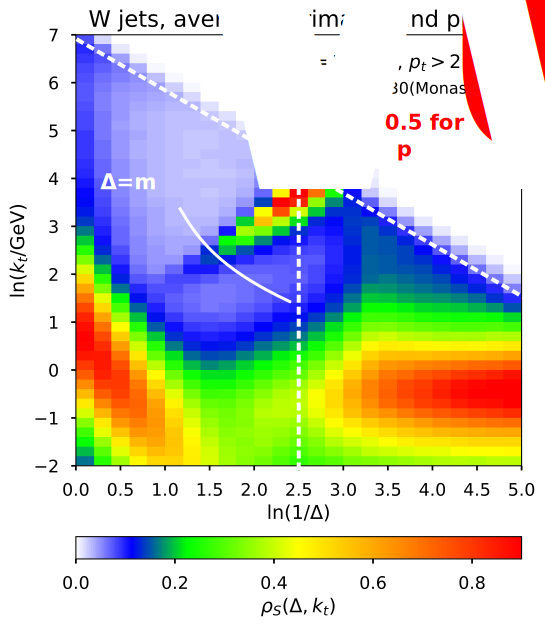
\includegraphics[width=0.6\textwidth]{05/wjetdm.pdf}
\end{center}
with $
\rho(\Delta,k_t) \equiv \frac{1}{N_\text{jet}}\frac{dn_\text{emissions}}{d\log(1/\Delta)d\log(k_t)}
$.
\end{frame}

\end{document}